% y = arsh(x)
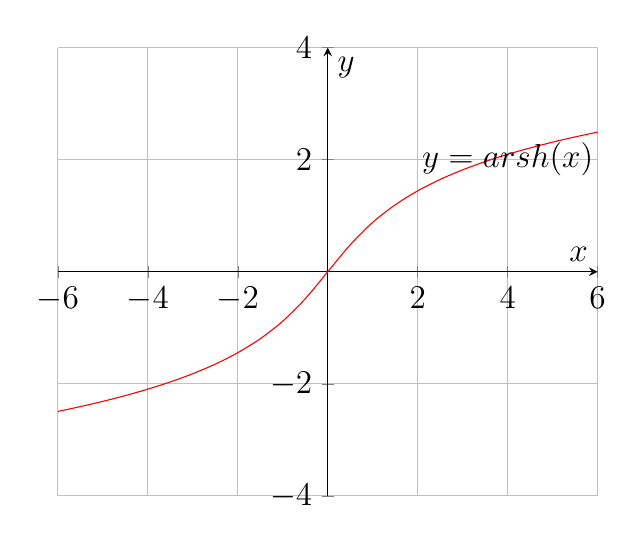
\begin{tikzpicture}
  \begin{axis}[domain=-6:6,ymin=-4,ymax=4, grid=both, font=\large, axis lines = middle, smooth, xlabel={$x$}, ylabel={$y$}]
    \addplot[draw=red] {ln(x + sqrt(x^2 + 1))};
    \node at (axis cs:4,2) {$y = arsh(x)$};
  \end{axis}
\end{tikzpicture}
